\documentclass[UTF8]{ctexart}  
\usepackage{graphicx}
\title{HW1}
\author{王嵘晟PB17111614}
\date{}
\begin{document}
\maketitle
\section*{2.1-1}
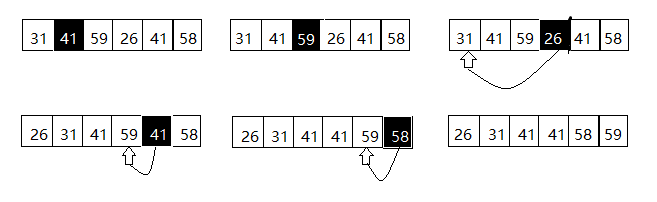
\includegraphics[scale=0.5]{HW1.png}
\section*{2.1-3}
    \noindent LEANER-SEARCH(A,v)
	\par\noindent{for i=1 to n}     
	\par{if A[i]=v}
	\par{return i}
	
	\noindent return NIL
	\\
	\\
    \noindent{A[1..i-1]是循环不变式}
    \par{初始化:第一次循环迭代之前(i=1)时循环不变式成立。子数组没有元素,所以v不等于子数组中任何元素的值,因此第一次循环迭代之前循环不变式成立。}
    \par 保持:for循环只对数组A[1..i]进行线性遍历检索,不对数组内容与顺序产生任何影响。子数组A[1..i]由原来在A[1..i]中的元素组成且顺序不变,且v不在A[1..i]中。对for循环的下一次迭代增加i将保持循环不变式。
    \par {终止:导致for循环终止的条件是}
    i \textgreater n
    。因为每次循环迭代i增加1,那么必有i=n+1。在循环不变式的表述中将i用n+1代替,则子数组A[1..n]由原来在A[1..n]中的元素组成且顺序不变,即为整个数组。因此算法正确。
\section*{2.2-3}
    \par {平均需要检查输入序列元素个数为}
    $$\frac{n+1}{2}$$
    \par 最坏情况查找元素个数为 \ n
    \\
    \par{由于要查找的元素是等可能的,则每个元素被查找的概率都为  $$ \frac{1}{n} $$ 则平均查找的运行时间为 $$ \sum_{1}^{n}\frac{i}{n}=\frac{n+1}{2}$$所以平均情况的运行时间为$\Theta(n)$}
    \par{最坏的情况是查找的元素在数组的最后一位或者根本不在数组中,此时对数组进行了完全遍历,此时运行时间为$\Theta(n)$}
\end{document}